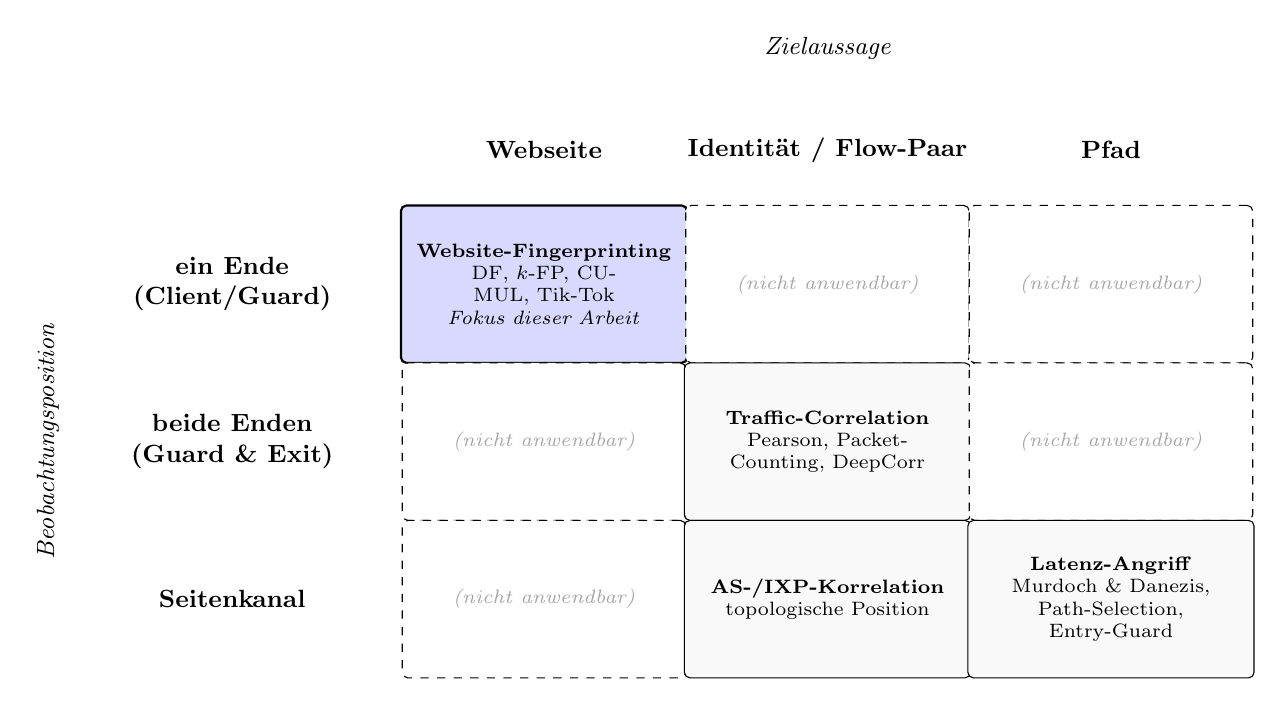
\begin{tikzpicture}[
    >=latex,
    every node/.style={font=\small},
    colheader/.style={
        align=center, font=\small\bfseries,
        minimum width=36mm, minimum height=8mm
    },
    rowheader/.style={
        align=center, font=\small\bfseries,
        minimum width=32mm, minimum height=20mm,
        text width=30mm
    },
    cell/.style={
        draw, rounded corners=2pt,
        minimum width=36mm, minimum height=20mm,
        align=center, fill=gray!5,
        text width=34mm, font=\scriptsize
    },
    focuscell/.style={
        draw, rounded corners=2pt, thick,
        minimum width=36mm, minimum height=20mm,
        align=center, fill=blue!15,
        text width=34mm, font=\scriptsize
    },
    emptycell/.style={
        draw, dashed, rounded corners=2pt,
        minimum width=36mm, minimum height=20mm,
        align=center, fill=white,
        font=\scriptsize\itshape, text=gray!70
    }
]

\def\cw{36mm}
\def\rh{20mm}

% Achsentitel oben (Zielaussage)
\node[font=\small\itshape] at (1*\cw, 2.5*\rh) {Zielaussage};

% Achsentitel links (Beobachtungsposition)
\node[font=\small\itshape, rotate=90] at (-1.75*\cw, 0) {Beobachtungsposition};

% Spaltenkoepfe
\node[colheader] at (0*\cw, 1.85*\rh) {Webseite};
\node[colheader] at (1*\cw, 1.85*\rh) {Identität / Flow-Paar};
\node[colheader] at (2*\cw, 1.85*\rh) {Pfad};

% Zeilenkoepfe
\node[rowheader] at (-1.1*\cw, 1*\rh)  {ein Ende\\(Client/Guard)};
\node[rowheader] at (-1.1*\cw, 0*\rh)  {beide Enden\\(Guard \& Exit)};
\node[rowheader] at (-1.1*\cw, -1*\rh) {Seitenkanal};

% Zeile 1: ein Ende
\node[focuscell] at (0*\cw, 1*\rh)
    {\textbf{Website-Fingerprinting}\\DF, $k$-FP, CUMUL, Tik-Tok\\\textit{Fokus dieser Arbeit}};
\node[emptycell] at (1*\cw, 1*\rh)  {(nicht anwendbar)};
\node[emptycell] at (2*\cw, 1*\rh)  {(nicht anwendbar)};

% Zeile 2: beide Enden
\node[emptycell] at (0*\cw, 0*\rh)  {(nicht anwendbar)};
\node[cell]      at (1*\cw, 0*\rh)
    {\textbf{Traffic-Correlation}\\Pearson, Packet-Counting, DeepCorr};
\node[emptycell] at (2*\cw, 0*\rh)  {(nicht anwendbar)};

% Zeile 3: Seitenkanal
\node[emptycell] at (0*\cw, -1*\rh) {(nicht anwendbar)};
\node[cell]      at (1*\cw, -1*\rh)
    {\textbf{AS-/IXP-Korrelation}\\topologische Position};
\node[cell]      at (2*\cw, -1*\rh)
    {\textbf{Latenz-Angriff}\\Murdoch \& Danezis,\\Path-Selection, Entry-Guard};

\end{tikzpicture}
